\chapter{\label{desarrollo}Desarrollo}

En este capítulo se describe el proceso técnico de creación de la aplicación, desde la gestión de los modelos tridimensionales hasta la arquitectura de la \gls{ui}. En primer lugar, se expone la propuesta de solución a nivel conceptual, detallando las funcionalidades integradas en el sistema. Posteriormente, se analizará cada parte de la implementación lógica y matemática que hace posible dichas herramientas.\footnote{Assets utilizados: Skybox menú principal (vista 360º) (\url{https://maps.app.goo.gl/Qa8RHXL4oYLrD1Km6}), skybox del resto de escenas (\url{https://assetstore.unity.com/packages/2d/textures-materials/sky/skybox-series-free-103633}) y tercer modelo de prueba (Apartamentos) (\url{https://www.nordicsustainableconstruction.com/knowledge/2024/august/bim4lca-files}).}

\section{Propuesta de Solución y Arquitectura General}

Para abordar los problemas de discrepancia entre el diseño teórico y la ejecución física en obra, se propone el desarrollo de un entorno de auditoría inmersivo en Realidad Virtual. Esta aplicación actúa como un puente entre la metodología BIM y la realidad construida, permitiendo a los operadores inspeccionar, validar y documentar el estado de un proyecto arquitectónico a escala real.

La solución se estructura en torno a un conjunto de herramientas interactivas que el usuario puede manejar de manera intuitiva mediante sus controladores. La propuesta principal engloba las siguientes funcionalidades clave:

\begin{itemize}
    \item \textbf{Visualización Dual:} Capacidad para transicionar instantáneamente entre el modelo teórico del edificio (diseño BIM) y una digitalización tridimensional fotorrealista del entorno real reconstruida volumétricamente.
    \item \textbf{Auditoría Geométrica mediante Escáner:} Herramienta de diagnóstico que proyecta un mapa de calor sobre las superficies, evaluando matemáticamente las desviaciones milimétricas entre lo construido y el plano original.
    \item \textbf{Medición Espacial Precisa:} Un sistema de cinta métrica virtual que permite calcular distancias exactas entre cualquier punto de la obra, facilitando la comprobación de dimensiones y tolerancias.
    \item \textbf{Detección Automática de Interferencias:} Módulo que evalúa las colisiones estructurales entre las instalaciones (conductos, tuberías) y la propia estructura del edificio (suelos, pilares...), aislando visualmente los conflictos para su resolución.
    \item \textbf{Inspección y Gestión Estructural:} Acceso a los metadatos y propiedades de cada elemento del diseño, con la posibilidad de "deconstruir" virtualmente el edificio ocultando capas arquitectónicas enteras o piezas de manera individual, por ejemplo, para ocultar paredes y ver las tuberías subyacentes.
    \item \textbf{Trazabilidad y Generación de Informes:} Sistema integrado que permite tomar fotografías virtuales, etiquetar incidencias por gravedad y compilar automáticamente toda la información recopilada en un documento \gls{pdf} exportable.
\end{itemize}

Para facilitar la comprensión global de la herramienta, en el siguiente diagrama (Cuadro~\ref{fig:arquitectura_propuesta}) se ilustra el flujo de trabajo principal de la aplicación y la disposición de las interfaces de usuario.

\begin{table}[!htb]
    \centering
    % Ajusta automáticamente el tamaño para que no se salga de los márgenes de la página
    \resizebox{\textwidth}{!}{%
    \begin{tikzpicture}[
        node distance=1.5cm and 1cm,
        font=\sffamily\small,
        % Estilos de las cajas
        base/.style={rectangle, draw=black!70, thick, rounded corners=2mm, align=center, minimum height=1.2cm, fill=white, drop shadow={opacity=0.25}},
        input/.style={base, fill=blue!10, text width=3.5cm},
        core/.style={base, fill=gray!15, text width=7cm, minimum height=1.5cm},
        tool/.style={base, fill=green!10, text width=3cm, minimum height=1.5cm},
        output/.style={base, fill=red!10, text width=5cm},
        group/.style={rectangle, draw=black!50, dashed, rounded corners=3mm, inner sep=15pt},
        arrow/.style={->, thick, draw=black!70, >=stealth}
    ]

    % 1. Nodos de Entrada (Inputs)
    \node[input] (bim) {\textbf{Modelo Teórico}\\(Diseño BIM)};
    \node[input] (real) [right=3cm of bim] {\textbf{Captura Física}\\(Gaussian Splatting)};

    % 2. Núcleo del sistema
    \node[core] (motor) [below=1.5cm of $(bim)!0.5!(real)$] {\textbf{Núcleo de Procesamiento}\vspace{1mm}\\Alineación Espacial y Físicas Procedurales};

    % 3. Herramientas de Auditoría
    \node[tool] (t1) [below left=2cm and 0.5cm of motor] {\textbf{Escáner}\\Mapa de Calor};
    \node[tool] (t2) [right=0.5cm of t1] {\textbf{Medición}\\Cinta Euclidiana};
    \node[tool] (t3) [right=0.5cm of t2] {\textbf{Colisiones}\\Clash Detection};
    \node[tool] (t4) [right=0.5cm of t3] {\textbf{Gestión}\\Capas y Metadatos};

    % Caja contenedora para agrupar las herramientas
    \node[group, fit=(t1) (t4), label={[font=\sffamily\bfseries, text=black!70]above:Módulos Analíticos e Interacción VR}] (herramientas) {};

    % 4. Salida de Datos
    \node[output] (pdf) [below=2cm of $(t2)!0.5!(t3)$] {\textbf{Generación de Informes}\\(Piezas BIM, Capturas e Incidencias)};

    % --- Trazado de Flechas de Conexión ---
    
    % Entradas al núcleo
    \draw[arrow] (bim) -- (motor);
    \draw[arrow] (real) -- (motor);

    % Núcleo a las herramientas
    \draw[arrow] (motor) -- (herramientas);

    % Punto de convergencia para las salidas
    \coordinate (merge) at ($(t2.south)!0.5!(t3.south) + (0,-1cm)$);
    
    % Flechas desde las herramientas al punto de convergencia
    \draw[arrow] (t1.south) |- (merge);
    \draw[arrow] (t2.south) |- (merge);
    \draw[arrow] (t3.south) |- (merge);
    \draw[arrow] (t4.south) |- (merge);
    
    % Flecha final al PDF
    \draw[arrow] (merge) -- (pdf.north);

    \end{tikzpicture}
    }
    \caption{Diagrama conceptual de la arquitectura de la aplicación y herramientas disponibles}
    \label{fig:arquitectura_propuesta}
\end{table}

A partir de este punto, se detallan los mecanismos lógicos y estructurales desarrollados para implementar cada una de estas propuestas.




\section{Configuración del Entorno de Desarrollo y SDK}

El inicio de la fase de desarrollo se caracterizó por ser un proceso directo y lineal.Debido a los estándares actuales de la industria para el despliegue de aplicaciones inmersivas, la puesta en marcha del proyecto dentro del motor gráfico de Unity, se siguieron los pasos de inicialización y configuración de dependencias documentados en la plataforma oficial del visor~\cite{metaquest2023}. Esta base documental facilitó la adopción de los estándares abiertos de realidad extendida, estableciendo un marco de trabajo sólido.

La integración del kit de desarrollo base provee una arquitectura modular compuesta por subsistemas esenciales, indispensables para cualquier experiencia de Realidad Virtual:

\begin{itemize}
    \item \textbf{Sistema de Cámara Estereoscópica y Rastreo Espacial:} Sustituye el renderizado tradicional por cámaras duales encargadas de generar la distorsión estereoscópica necesaria para percibir la profundidad. Este componente traslada los movimientos de la cabeza del operario al espacio virtual de forma instantánea.
    \item \textbf{Controles de Entrada y Mapeo de Dispositivos:} Subsistema que extrae las señales de hardware provenientes de los controladores en eventos lógicos, permitiendo la lectura precisa de botones, superficies táctiles y gatillos.
    \item \textbf{Interactores y Componentes de Selección:} Módulos que gestionan las mecánicas de interacción, proveyendo herramientas nativas para la manipulación directa por proximidad y la selección a distancia mediante punteros virtuales (raycast).
    \item \textbf{Físicas y Capas de Colisión:} Reglas del motor que controlan la gravedad artificial y delimitan las áreas transitables.
\end{itemize}

Esta infraestructura base actúa como el núcleo técnico del proyecto, garantizando que el visor procese el movimiento de manera óptima antes de abordar las herramientas analíticas especializadas de la aplicación.

\section{Generación Procedural de Físicas y Optimización}

Para que las herramientas de interacción a distancia —como el escáner de mapa de calor o el puntero de selección— operen de forma precisa sobre el modelo arquitectónico, es necesario que cada elemento geométrico posea un volumen físico capaz de registrar impactos. Configurar esto de forma manual en modelos complejos que contienen miles de piezas resulta inviable.

Para automatizar este proceso, se desarrolló un algoritmo de optimización que opera durante la inicialización del entorno. Este sistema utiliza una rutina de procesamiento asíncrono para iterar sobre todas las mallas visuales del edificio. Al detectar una pieza que no tenga propiedades físicas, el sistema le adhiere dinámicamente un volumen de colisión y le transfiere la topología exacta del objeto tridimensional.

Con el objetivo mantener estabilidad en la tasa de fotogramas y prevenir interrupciones en el seguimiento del visor, la ejecución se ha escalonado mediante pausas controladas. Al introducir un nuevo colisionador, el hilo principal de procesamiento se detiene forzando un fotograma de espera de forma inmediata, mitigando así picos severos en la carga computacional. En caso de que la pieza evaluada ya cuente con propiedades físicas preexistentes, el algoritmo continúa la inspección secuencial introduciendo de manera preventiva una pausa de un fotograma cada 100 comprobaciones para liberar el flujo de datos del sistema. En el Cuadro~\ref{diagrama_optimizacion} se detalla de forma exhaustiva la lógica de control y bifurcación de este algoritmo concurrente.

\begin{table}[!htb]
    \centering
    \resizebox{0.95\textwidth}{!}{%
    \begin{tikzpicture}[
        node distance=1cm and 1.2cm,
        font=\sffamily\small,
        % Estilos de las cajas
        base/.style={rectangle, draw=black!70, thick, rounded corners=2mm, align=center, minimum height=1.2cm, fill=white, drop shadow={opacity=0.25}},
        main/.style={base, fill=blue!10, text width=3.5cm},
        process/.style={base, fill=gray!15, text width=4.8cm},
        decision/.style={diamond, draw=black!70, thick, fill=yellow!10, align=center, inner sep=0pt, text width=2.6cm, aspect=1.4, drop shadow={opacity=0.25}},
        wait/.style={base, fill=orange!10, text width=3.2cm, dashed},
        group/.style={rectangle, draw=black!50, dashed, rounded corners=3mm, inner sep=12pt},
        arrow/.style={->, thick, draw=black!70, >=stealth},
        line/.style={thick, draw=black!70}
    ]

    % Nodos Centrales e Iniciales
    \node[main] (start) {\textbf{Hilo Principal}\\(Inicio de Escena)};
    \node[process] (get) [below=0.8cm of start] {\textbf{Extracción de Datos}\\Obtener listado de mallas visuales};
    \node[decision] (collider) [below=0.8cm of get] {¿Tiene\\colisionador?};

    % Coordenadas absolutas para alinear la altura
    \node[process] (add) at ([xshift=-2.6cm, yshift=-2.6cm]collider.south) {\textbf{Generación de Físicas}\\Adherir MeshCollider};
    \node[decision] (count100) at ([xshift=2.8cm, yshift=-2.6cm]collider.south) {¿Múltiplo de\\100 iteraciones?};

    \node[wait] (yield_add) [below=0.8cm of add] {\textbf{Pausa Forzada}\\(Espera 1 fotograma)};
    \node[wait] (yield_count) [below=0.8cm of count100] {\textbf{Pausa de Control}\\(Espera 1 fotograma)};

    % Se baja el nodo loop para dar más margen a la unión
    \coordinate (loop_y) at ([yshift=-1.8cm]yield_count.south);
    \node[decision] (loop) at (collider |- loop_y) {¿Faltan mallas\\por evaluar?};

    % Puntos de anclaje para enrutar flechas por FUERA de todos los nodos
    \coordinate (leftPath) at ([xshift=-1.4cm]add.west);
    \coordinate (rightPath) at ([xshift=1.4cm]count100.east);

    % Nodo Final
    \node[main] (end) [below=1.2cm of loop] {\textbf{Hilo Principal}\\(Interacción del usuario)};

    % Caja contenedora
    \node[group, fit=(collider) (add) (yield_add) (count100) (yield_count) (loop) (leftPath) (rightPath), label={[font=\sffamily\bfseries, text=black!70]above left:Rutina de Procesamiento Asíncrono}] (rutina) {};

    % ---------------- ENRUTAMIENTO DE FLECHAS ---------------- %

    \draw[arrow] (start) -- (get);
    \draw[arrow] (get) -- (collider);

    % Bifurcación limpia
    \coordinate (fork_collider) at ([yshift=-0.6cm]collider.south);
    \draw[line] (collider.south) -- (fork_collider);
    \draw[arrow] (fork_collider) -| node[above, pos=0.25] {No} (add.north);
    \draw[arrow] (fork_collider) -| node[above, pos=0.25] {Sí} (count100.north);

    % Bajada desde la rama izquierda
    \draw[arrow] (add) -- (yield_add);

    % Bajada desde la rama derecha
    \draw[arrow] (count100.south) -- node[right] {Sí} (yield_count.north);

    % By-pass derecho
    \draw[arrow] (count100.east) -- node[above] {No} (rightPath |- count100.east) |- (loop.east);

    % Unión forzada explícitamente por debajo de los nodos para evitar cruces
    \coordinate (join_y) at ([yshift=-0.8cm]yield_add.south);
    \coordinate (join_center) at (collider |- join_y);
    
    \draw[line] (yield_add.south) |- (join_center);
    \draw[line] (yield_count.south) |- (join_center);
    \draw[arrow] (join_center) -- (loop.north);

    % Salida del bucle
    \draw[arrow] (loop.south) -- node[right] {No} (end.north);

    % Retorno del bucle
    \draw[arrow] (loop.west) -- node[above] {Sí} (leftPath |- loop.west) -- (leftPath |- collider.west) -- (collider.west);

    \end{tikzpicture}
    }
    \caption{Diagrama de flujo del proceso asíncrono para la generación de físicas}
    \label{diagrama_optimizacion}
\end{table}


\section{Gestión Dual de Modelos y Visualización}

La aplicación permite al usuario alternar dinámicamente entre el modelo de diseño teórico y la captura física de la realidad. Esto es fundamental para identificar discrepancias visuales de forma rápida. Para gestionar esta funcionalidad, se desarrolló un controlador lógico basado en una máquina de estados que define tres modalidades de visualización: exclusiva para el diseño, exclusiva para la realidad escaneada, o una superposición de ambas.

El sistema evalúa continuamente las pulsaciones de los botones del usuario. Al recibir la orden de cambio, el controlador recalcula qué modelo debe ser visible y altera el estado de activación en la jerarquía del entorno. Cabe destacar que, para el renderizado del modelo físico, se implementó un forzado de actualización sobre el buffer de la memoria gráfica al volver a un estado activo, asegurando que las partículas volumétricas se redibujen sin errores visuales tras un periodo ocultas.

La integración de este sistema se realizó mediante un objeto gestor centralizado en la arquitectura del proyecto, el cual mantiene las referencias en memoria de ambos ecosistemas tridimensionales, tal como se aprecia en la Figura~\ref{fig:layer-switcher-unity}.

\begin{figure}[!htb]
    \centering
    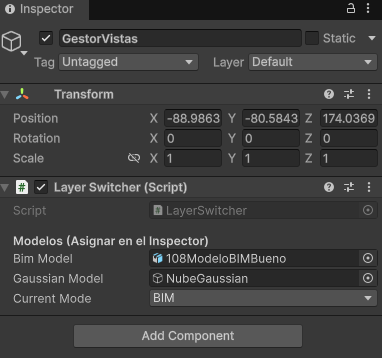
\includegraphics[width=0.7\linewidth]{include/images/figura5.1.png}
    \caption{Configuración del gestor de visualización en el motor de desarrollo}
    \label{fig:layer-switcher-unity}
\end{figure}


\section{Alineación Espacial de Modelos (Diseño vs Realidad)}

Para que el diagnóstico de desviaciones funcione correctamente, es indispensable que el modelo teórico de diseño y la reconstrucción tridimensional del edificio real compartan el mismo sistema de coordenadas globales. Dado que las capturas de la realidad suelen generarse con orígenes arbitrarios, se desarrolló un sistema matemático para automatizar la superposición precisa de ambos entornos.

El sistema emplea un algoritmo de emparejamiento basado en tres puntos de referencia homólogos definidos en ambos espacios:
\begin{itemize}
    \item \textbf{Punto 1 (Origen):} Define la traslación espacial exacta entre ambos mundos.
    \item \textbf{Punto 2 (Dirección Frontal):} Establece el vector de profundidad y la orientación cardinal.
    \item \textbf{Punto 3 (Dirección Superior):} Define el plano de apoyo y el vector de verticalidad.
\end{itemize}

Matemáticamente, el algoritmo calcula los vectores directores de orientación utilizando el producto vectorial entre las tres referencias establecidas. Con estos datos, el sistema determina la diferencia espacial de rotación existente y aplica de forma automática la transformación geométrica pertinente sobre el modelo escaneado. Esta corrección toma como referencia el punto de origen, logrando coincidir ambos modelos (Figura~\ref{fig:alineador}).

\begin{figure}[!htb]
    \centering
    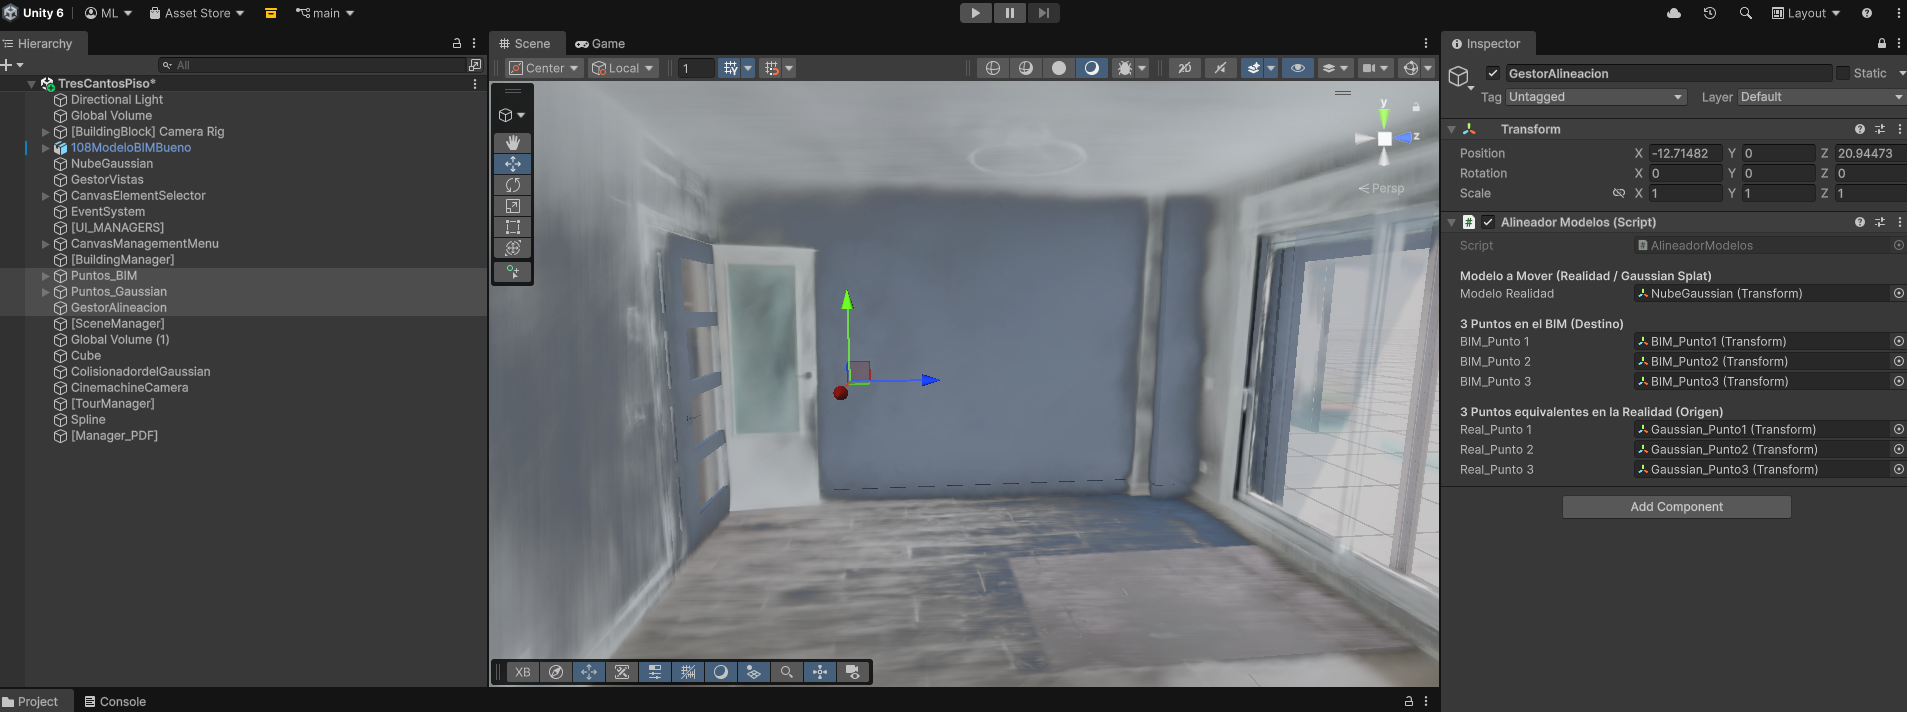
\includegraphics[width=0.8\linewidth]{include/images/figura5.7.png}
    \caption{Modelos alineados de forma automática}
    \label{fig:alineador}
\end{figure}

\section{Detección Automática de Colisiones}

Una de las fases más críticas en la coordinación de obras es la identificación de interferencias entre las instalaciones (conductos, tuberías) y los elementos estructurales (Figura~\ref{fig:MEP-struct}). Para automatizar este proceso, se implementó un módulo que evalúa las colisiones mediante la intersección de cajas delimitadoras tridimensionales.

Para evitar falsos positivos causados por roces superficiales (elementos que están en contacto válido pero no se atraviesan), el sistema realiza una reducción matemática de los límites de estas cajas antes de la evaluación. Si tras esta substracción los volúmenes se siguen intersecando, se confirma un conflicto estructural crítico.

Al detectar una interferencia, el sistema ejecuta tres acciones automatizadas:
\begin{enumerate}
    \item Instancia de manera procedural un marcador visual esférico en el centro exacto de la colisión, calculado a partir del promedio espacial de la superposición.
    \item Registra el impacto en el registro de datos global para su posterior volcado en el sistema de informes.
    \item Se comunica con el gestor de capas arquitectónicas enviando un conjunto de datos con las piezas involucradas. El sistema aísla automáticamente estos elementos, ocultando el resto del edificio para proporcionar al usuario una vista despejada del problema.
\end{enumerate}

\begin{figure}[!htb]
    \centering
    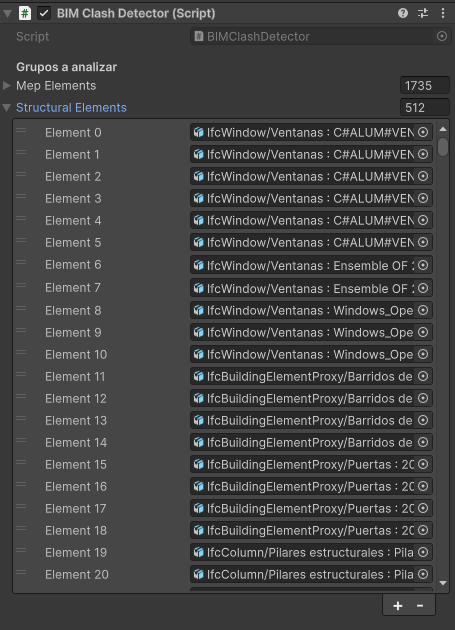
\includegraphics[width=0.8\linewidth]{include/images/figura5.8.png}
    \caption{Elementos divididos entre estructurales e instalaciones (MEP)}
    \label{fig:MEP-struct}
\end{figure}



\section{Sistema de Punteros e Interacción a Distancia}

En Realidad Virtual, el usuario necesita una referencia visual constante que indique la orientación de sus controladores para interactuar con interfaces o elementos distantes. Para lograrlo, se implementó un sistema de proyección que simula un "puntero láser".

El módulo calcula una línea poligonal continua en el espacio 3D. En cada iteración gráfica, el algoritmo toma la posición física de la mano del usuario como punto de origen y calcula un vector proyectado hacia adelante multiplicado por una constante de distancia. Para evitar que el rayo se comporte de forma errática al rotar la muñeca, se forzó el cálculo de los vértices sobre el espacio de coordenadas globales de la escena en lugar del local de la mano.

El láser resultante se renderizó con un grosor mínimo para simular precisión milimétrica, y se le aplicó un material puro sin cálculo de iluminación o sombras, garantizando que el haz de luz mantenga su visibilidad máxima sin importar las condiciones de oscuridad de la obra virtual. Como podemos observar en la Figura \ref{fig:rayvisual}, el rayo de cada controlador es distinto, al ser el izquierdo para seleccionar piezas es más grueso, y el derecho, al requerir un control más preciso es más fino.

\begin{figure}[!htb]
    \centering
    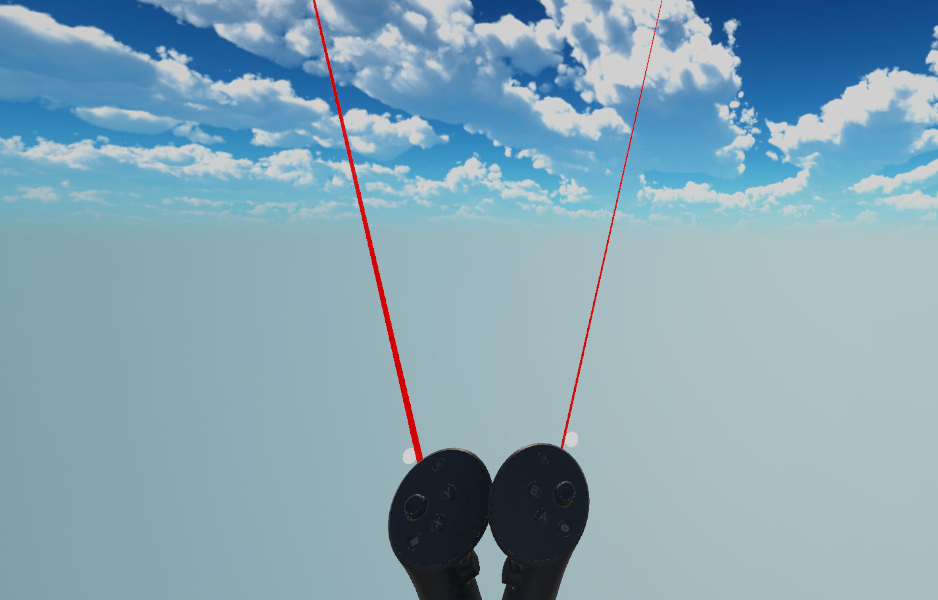
\includegraphics[width=0.8\linewidth]{include/images/controllerrayvisual.png}
    \caption{Raycast de cada controlador}
    \label{fig:rayvisual}
\end{figure}



\section{Inspección de Metadatos y Deconstrucción Selectiva}

El sistema permite apuntar a piezas individuales del diseño, extraer su información técnica (categoría, nombre de sistema, identificador) y visualizarla en un panel flotante (Figura \ref{fig:inspeccion}. Además, incluye la capacidad de ocultar el elemento seleccionado para visualizar el interior de las estructuras.

El algoritmo lanza un rayo físico invisible desde el mando que es filtrado mediante máscaras lógicas para asegurar que solo interactúa con geometría del edificio a inspeccionar. Al colisionar, se activa un retroalimentador visual que cambia el color de la pieza. El módulo de inspección fragmenta los datos del elemento objetivo para reconstruir una ficha técnica con formato legible.

El gestor de la interfaz calcula dinámicamente la posición del panel de información basándose en vectores espaciales. El panel se sitúa siempre a una distancia prudencial frente al usuario y se orienta hacia su línea de visión, garantizando la legibilidad (Figura~\ref{fig:ovr-controllers-unity}). El usuario puede ocultar la pieza inspeccionada mediante un comando directo, y el sistema memoriza estos elementos en una estructura de datos para permitir su restauración total mediante otro atajo en los controladores.

\begin{figure}[!htb]
    \centering
    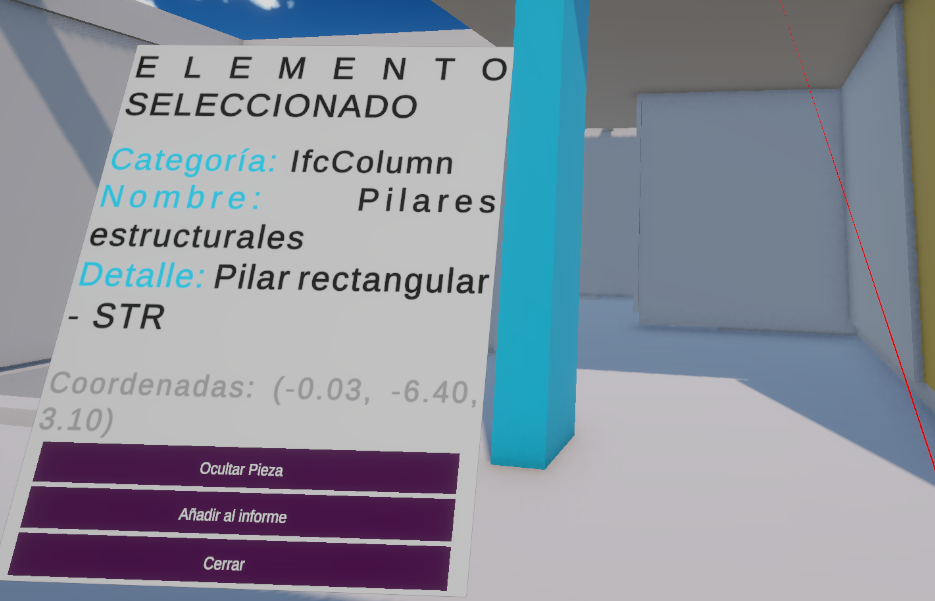
\includegraphics[width=0.8\linewidth]{include/images/inspeccion.png}
    \caption{Interfaz mostrada al inspeccionar una columna de manera individual}
    \label{fig:inspeccion}
\end{figure}

\begin{figure}[!htb]
    \centering
    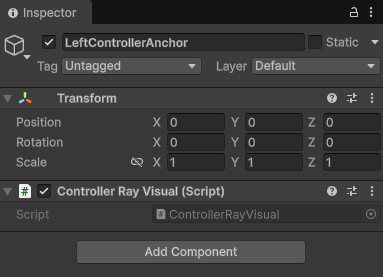
\includegraphics[width=0.5\linewidth]{include/images/figura5.2.png}
    \caption{Integración del sistema de control y selección de elementos en el entorno}
    \label{fig:ovr-controllers-unity}
\end{figure}

Para dotar a la herramienta de trazabilidad, el módulo de selección se integra con el motor documental. Al inspeccionar una pieza, el sistema evalúa si ya forma parte del registro de la auditoría. De no ser así, habilita una opción para registrar el elemento con sus coordenadas para su posterior exportación.


\subsection{Inteligencia Espacial y Prevención de Oclusiones}

Desplegar interfaces flotantes a una distancia estática presentaba un riesgo de oclusión severo: si el usuario inspeccionaba un elemento muy cercano a un muro, el panel atravesaba la pared física, imposibilitando su lectura. 

Para dotar a la interfaz de consciencia espacial, el sistema implementa un algoritmo de seguridad dinámico. Antes de hacer aparecer el menú, se proyecta un rayo desde los ojos del usuario hacia la coordenada ideal del panel, buscando intersecciones con elementos estructurales. Si se detecta un obstáculo, el algoritmo acorta matemáticamente el vector de distancia, reubicando la interfaz justo antes del punto de impacto. Se estableció además un límite de cercanía mínima absoluta para evitar problemas de enfoque ocular y fatiga visual.




\section{Herramienta de Medición Espacial Euclidiana}

Para evaluar discrepancias, el usuario cuenta con una "cinta métrica virtual" capaz de calcular distancias exactas entre cualquier par de puntos del espacio tridimensional a partir del modelo teórico. Visto en la Figura \ref{fig:informe-diseño}.

El sistema de medición opera mediante una máquina de estados controlada por las interacciones del operario:
\begin{enumerate}
    \item \textbf{Apuntado Inicial:} Se proyecta un láser secundario constante que indica el punto exacto de colisión física sobre las superficies, ignorando mediante un sistema de capas las interfaces flotantes para evitar mediciones erróneas.
    \item \textbf{Fijación del Primer Punto:} Al registrar la primera pulsación, se captura la coordenada tridimensional de origen. La cinta visual se ancla en este punto y se estira dinámicamente siguiendo la orientación de la mano del usuario.
    \item \textbf{Fijación del Segundo Punto:} Una segunda pulsación confirma la coordenada de destino. El algoritmo resuelve la distancia euclidiana exacta entre ambos puntos en el espacio. Esta medición se inyecta inmediatamente en la memoria de la sesión para el informe de auditoría.
    \item \textbf{Representación Visual:} Se genera dinámicamente un indicador de texto flotante que se sitúa en el punto medio geométrico exacto del segmento trazado, mostrando el valor métrico resultante.
\end{enumerate}




\section{Registro de Incidencias y Trazabilidad}

La aplicación provee un sistema para señalar problemas visuales manualmente y categorizarlos mediante marcadores espaciales (Grave, Leve o a Revisar, Figura \ref{fig:incidencia}), utilizando un flujo de trabajo optimizado para no interrumpir la inmersión.

Para no saturar la aplicación, en lugar de utilizar menús, la selección de la gravedad de la incidencia se realiza mediante la lectura del eje direccional del controlador derecho (arriba, izquierda o derecha), bloqueando el giro de la cámara hecho con el mismo. Al clavar la marca de incidencia en el entorno, se adjunta información textual. Para garantizar que estos marcadores sean siempre legibles desde cualquier ángulo de la sala, se implementó una rutina matemática de orientación continua (\textit{Billboarding}), la cual fuerza la rotación geométrica de las etiquetas para que encaren constantemente el vector de visión del usuario.

\begin{figure}[!htb]
    \centering
    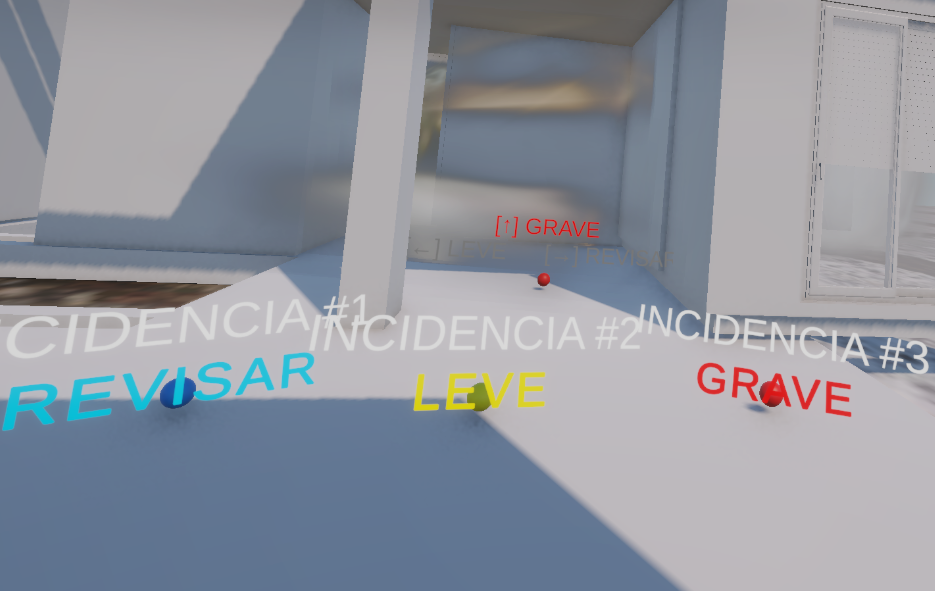
\includegraphics[width=0.8\linewidth]{include/images/incidencias.png}
    \caption{Niveles de incidencia posibles}
    \label{fig:incidencia}
\end{figure}


\section{Gestión y Filtrado de Tipologías Estructurales}

En la auditoría constructiva es habitual que más de un elemento superficial oculte sistemas críticos. Se desarrolló una herramienta de "deconstrucción" global que permite aislar o alterar la visibilidad de grupos enteros de elementos (como "Muros" o "Estructura") de forma masiva.

El sistema utiliza contenedores lógicos que agrupan listas de elementos tridimensionales según su tipología. Al arrancar, el sistema analiza el estado visible real del edificio. Posteriormente, permite ejecutar funciones de alternancia de visibilidad que iteran rápidamente sobre cientos de elementos para apagarlos o encenderlos simultáneamente. 

Dado que los controladores físicos tienen botones limitados, el mando sobre este sistema se delegó a una interfaz gráfica inmersiva, colocado cerca del punto de aparición del usuario. Cada categoría arquitectónica está vinculada a un botón bidimensional que envía la orden de visibilidad al contenedor correspondiente (Figura~\ref{fig:btn-capas-unity}).

\begin{figure}[!htb]
    \centering
    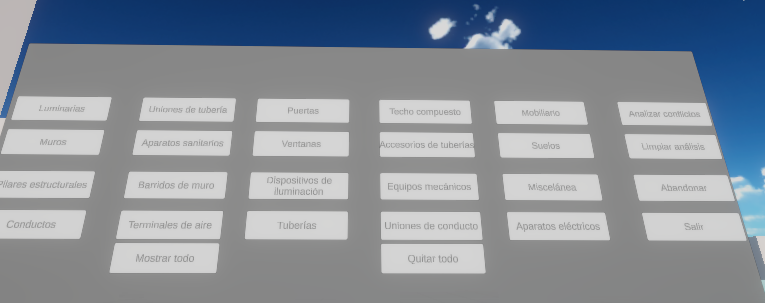
\includegraphics[width=0.8\linewidth]{include/images/figura5.3.png}
    \caption{Panel de gestión de capas estructurado en la interfaz inmersiva}
    \label{fig:btn-capas-unity}
\end{figure}



\section{Navegación e Interfaz Responsiva}

Para dotar a la aplicación de escalabilidad, se implementó un sistema de navegación entre diferentes modelos de edificios partiendo desde una sala central. El desafío técnico principal consistía en evitar que la manipulación de los menús activase accidentalmente las herramientas de auditoría.

Se implementó un sistema de exclusión basado en máscaras de colisión. El algoritmo detecta si el puntero láser está impactando sobre un elemento de la interfaz; de ser así, levanta una bandera lógica que desactiva temporalmente las herramientas métricas y de selección del entorno, enfocando las acciones del usuario exclusivamente hacia la navegación del menú.

Además, el láser visual se adaptó de forma dinámica: el haz de luz ahora calcula la distancia al primer objeto o sólido en su trayectoria y trunca su longitud en el punto de impacto, eliminando la ilusión óptica de un rayo que atraviesa las pantallas físicas. Los menús inmersivos reaccionan al tacto virtual modificando su color para que sean responsivas (Figura~\ref{fig:interfaz-menu}).

\begin{figure}[!htb]
    \centering
    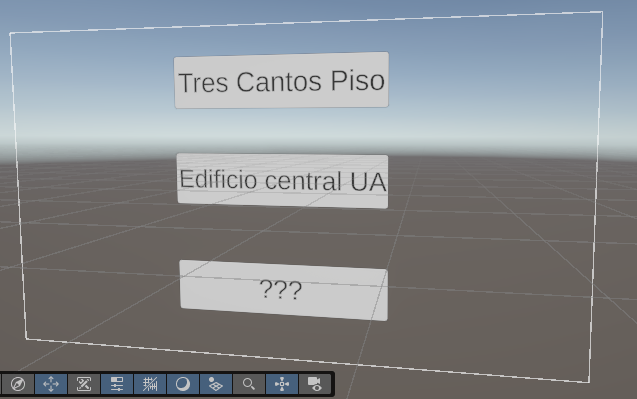
\includegraphics[width=0.8\linewidth]{include/images/figura5.4.png}
    \caption{Interfaz principal del menú y sistema de botones responsivos}
    \label{fig:interfaz-menu}
\end{figure}



\section{Interacciones y Prevención de Cinetosis}

Los cambios abruptos en el entorno virtual pueden romper la inmersión e inducir mareos. Para mitigarlo, se desarrolló un sistema de animaciones procedurales basadas en interpolación matemática. La aparición de menús u ocultación de elementos arquitectónicos no se produce de forma instantánea, sino alterando gradualmente su escala tridimensional. A esta transición se le aplicó una interpolación para que se sienta menos errático.

A la hora de interactuar con paneles virtuales, las herramientas estándar de Unity ofrecían una respuesta visual pobre. Se diseñó un módulo que reemplaza por completo el material de los botones al ser pulsados. Al realizar un intercambio de la propia textura en lugar de tintar la imagen, se respetan las sombras y brillos del entorno tridimensional, mejorando la respuesta táctil visual.

Para evitar mareos durante los tiempos de carga entre diferentes modelos arquitectónicos, las transiciones se delegaron a hilos de procesamiento en segundo plano, y se sincronizaron con un oscurecimiento progresivo de la visión del usuario. Esto garantiza que el seguimiento de los movimientos de la cabeza nunca se congele mientras el procesador prepara el nuevo entorno. Este oscurecimiento se logró creando un panel negro de gran tamaño delante de la cámara del usuario usuario (Figura~\ref{fig:camara}), que se hace visible progresivamente al cambiar de escena.

\subsection{Persistencia Local de Sesiones}
Se integró un sistema de almacenamiento ligero en la memoria del dispositivo que registra fechas y datos de inspección mediante cadenas de texto. Esta información se inyecta en la sala inicial, permitiendo al usuario llevar un control visual de las auditorías previas sin requerir complejas infraestructuras de bases de datos externas. Visto en la Figura \ref{fig:res-menu}.

\subsection{Desplazamiento Físico en Desniveles}
El desplazamiento por una maqueta implica subir o bajar escaleras. La simulación de gravedad estándar generaba caídas abruptas y micro-saltos al caminar rápidamente por un desnivel negativo. Para subsanarlo, el algoritmo aísla el cálculo de movimiento horizontal del vertical. Al detectar el borde de un escalón, el sistema realiza una presión vertical que actúa como un ancla magnética hacia la malla de las escaleras, forzando a descender adherido a la pendiente del peldaño y resultando en un tránsito fluido.




\section{Registro Documental y Generación de Informes}

Se implementó un sistema automático para documentar de manera visual y paramétrica las anomalías, el cual se divide en un subsistema de fotografía inmersiva y un motor de maquetación.

\subsection{Cámara Virtual Inmersiva}
Para capturar evidencias en obra, se desarrolló una herramienta que simula una cámara anclada a la mano del usuario, renderizando la perspectiva en una textura dinámica en tiempo real (Figura~\ref{fig:camara}). Al accionar el disparador, el algoritmo extrae la matriz de píxeles resultante, la codifica en un formato de imagen convencional y la almacena en el disco duro del visor. El proceso se acompaña de un efecto visual de destello sobre las lentes para confirmar la captura.

\begin{figure}[!htb]
    \centering
    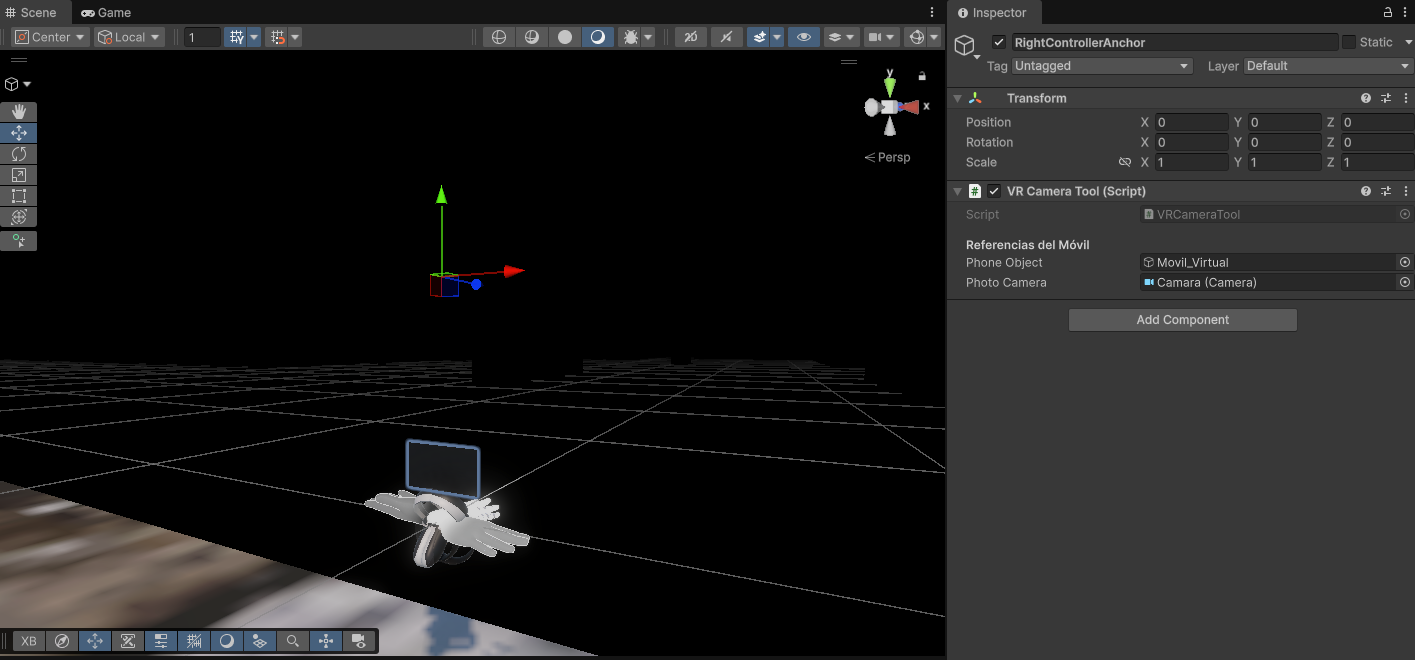
\includegraphics[width=0.8\linewidth]{include/images/figura5.10.png}
    \caption{Visualización inmersiva de la cámara para la captura de evidencias}
    \label{fig:camara}
\end{figure}

\subsection{Motor de Compilación de Datos}
La automatización del informe documental consiste en una arquitectura de memoria centralizada. Todas las herramientas de la aplicación operan independientemente, pero vuelcan sus hallazgos en estructuras de datos globales. Al solicitar la exportación, un motor basado en librerías de procesamiento de documentos organiza estos datos y diagrama en un archivo PDF.

Para una buena presentación, se encapsula lógicamente cada captura fotográfica junto a su texto descriptivo, forzando saltos de página inteligentes para evitar que queden huérfanos o separados. Tras compilar el archivo (Figura~\ref{fig:informe-diseño}), el sistema hace una limpieza de memoria, permitiendo realizar múltiples auditorías sucesivas sin reiniciar el programa.

\begin{figure}[!htb]
    \centering
    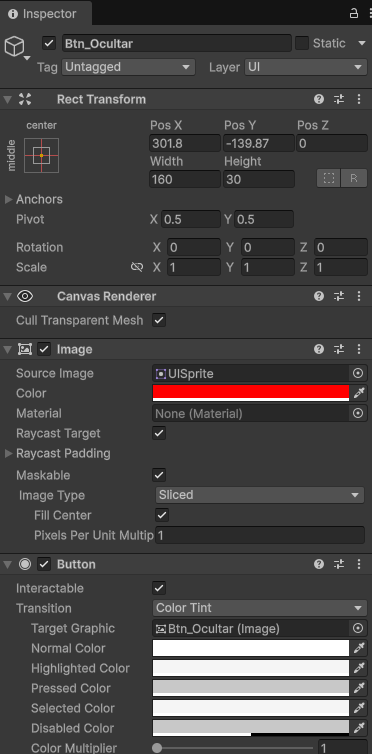
\includegraphics[width=0.8\linewidth]{include/images/figura5.5.png}
    \caption{Documento de auditoría final generado autónomamente por el sistema}
    \label{fig:informe-diseño}
\end{figure}






\section{Evaluación Volumétrica y Mapa de Calor Espacial}

Otra de las funciones de la aplicación para analizar es un escáner capaz de medir las diferencias entre la estructura real física y el modelo teórico en tiempo real. Esta herramienta tiñe los elementos del edificio teórico con un mapa de calor proyectado.

El desafío principal radicaba en que las digitalizaciones de la realidad carecen de volumen sólido, y procesar millones de partículas simultáneamente saturaría el procesador, volviendo la experiencia injugable. Para solucionarlo, el modelo volumétrico crudo se preprocesó mediante software especializado (CloudCompare) aplicando un submuestreo espacial, reduciendo considerablemente la densidad de puntos y aligerando el volumen de datos. Este modelo se exportó como documento de texto incluyendo todo el conjunto de puntos como coordenadas con el objetivo de optimizar el proceso y hacer posible esa comparación. A modo de prueba y validación, en la Figura \ref{fig:comparacion} se observa que los puntos cianes representan la versión simplificada del modelo con Gaussian Splat

\subsection{Algoritmo de Proximidad Topológica}
La herramienta de escáner ejecuta un cálculo de búsqueda espacial. Al interactuar con un muro teórico, el sistema analiza las coordenadas circundantes y evalúa la distancia hacia los puntos del modelo preprocesado.

Si el algoritmo confirma la existencia de masa física real dentro de un radio de tolerancia, verifica la validez de esa parte de la estructura.

\subsection{Clasificador de Desviaciones}
Esta evaluación se procesa a través de un sistema de clasificación gradual que analiza la magnitud del error detectado y altera en consecuencia la coloración de la superficie analizada:
\begin{itemize}
    \item \textbf{Verde (Perfecto):} Desviación ínfima. La obra física coincide íntegramente con el plano.
    \item \textbf{Amarillo (Aceptable):} Discrepancia leve pero asumible dentro de las tolerancias normales.
    \item \textbf{Naranja (Desviación Notable):} Error de ejecución evidente que requiere una revisión técnica.
    \item \textbf{Rojo (Fallo Crítico):} Ausencia total del elemento o desplazamiento que excede cualquier margen de seguridad permitido.
\end{itemize}

El resultado final es un diagnóstico inmersivo inmediato que, además de colorear la maqueta virtual (Figura~\ref{fig:comparacion}), registra cada comprobación para adjuntarla al informe global de la sesión.

\begin{figure}[!htb]
    \centering
    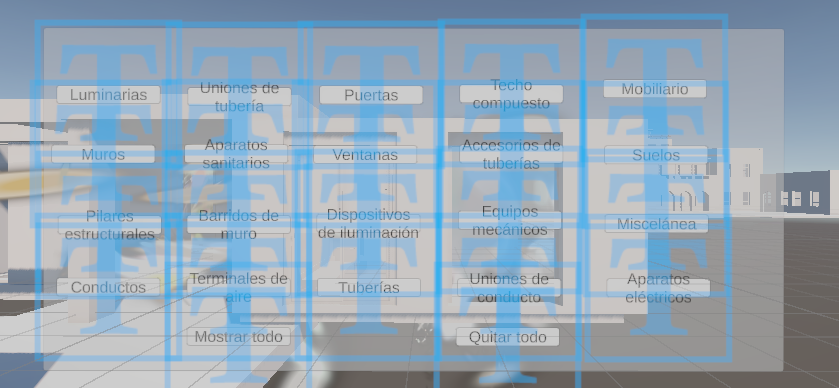
\includegraphics[width=0.8\linewidth]{include/images/figura5.6.png}
    \caption{Versión inicial del spray de mapa de calor con el modelo de puntos simplificado, inicialmente eran solo dos colores}
    \label{fig:comparacion}
\end{figure}